\chapter{Ordenando metadatos y aplicando algoritmos propuestos}

En este cap'itulo se har'a muestra de las t\'ecnicas necesarias para obtener la estructura de una base de datos, una base de datos existente por lo general lleva tablas que de alguna manera se relacionan entre ellas. El detallar la estructura de una base de datos comprende:
\begin{itemize}
\item Listar todas las tablas de una base de datos.
\item Listar las tablas que hacen referencia y a que tablas.
\item Listar las llaves primarias de una tabla.
\item Listar las llaves for\'aneas de una tabla.
\item Detallar los atributos de una tabla como ser el tipo de dato, tama\~no, si puede ser nulo. 
\end{itemize} 
Es muy importante realizar lo listado anteriormente para obtener la estructura de una base de datos, y usar estos resultados para construir una interfaz gr\'afica de configuraci\'on de generaci\'on de datos de acuerdo a las caracter\'isticas de la columna de una tabla.
Obtener la estructura de una base de datos puede variar dependiendo del DBMS(Database Managment System) con la que se trabaja, entre los DBMS se tiene a varios, las mas usadas son MySQL, PostgreSQL, Oracle, SQLServer y otras. En este proyecto se hace la eleccion de  trabajar con postgresSQl las razones para esta elecci\'on son las siguientes.
\begin{itemize}
\item Soporta llaves primarias compuestas(lo cual permite aplicar patrones de dise\~no ER Idioms).
\item Es un DBMS de licencia BSD libre.
\end{itemize}
Esto no significa que en las otras no se pueda aplicar este proyecto de lo contrario son aplicables a DBMS relacionales claro que existen diferencias de como manejan los datos internamente cada una de ellas, se puede mencionar que postgreSQL almacena en metadatos todas las tablas que se crea, por lo tanto se deduce que para obtener la estructura de una base de datos es necesario trabajar con metadatos de postgreSQL.
\section{Metadatos en PostgreSQL}
PostgreSQL tiene una arquitectura que involucra muchos estilos, en su nivel mas alto es un esquema cl\'asico cliente-servidor, mientras que el acceso a metadatos es un esquema en capas como se observa en la Figura \ref{fig:ArquitecturaPostgres} donde:

\begin{itemize}
\item Libpq es el responsable de manipular las comunicaciones entre la aplicaci\'on cliente y el postmaster(Servicio del PostgreSQL en el servidor).
\item El servidor esta compuesto por dos grandes subsistemas, ``Postmaster" que es el responsable de aceptar las comunicaciones con el cliente, autentificar y dar acceso. ``Postgre" se encarga de la administraci\'on de los consultas(querys) y comandos enviados por el cliente. PostgreSQL trabaja bajo el concepto de ``process per user", eso significa un solo proceso cliente por conexi\'on. Tanto el Postmaster como el ``Postgre" deben estar junto en el mismo servidor siempre.
\item El gestor de almacenamiento (Storage Manager) es responsable de la administraci\'on general del almacenamiento de los datos, controla todos los trabajos del back end incluido la administraci\'on del buffer, archivos, bloqueos y control de consistencia de la informaci\'on.   
\end{itemize}
\begin{figure}[H]
\centering
\subfigure{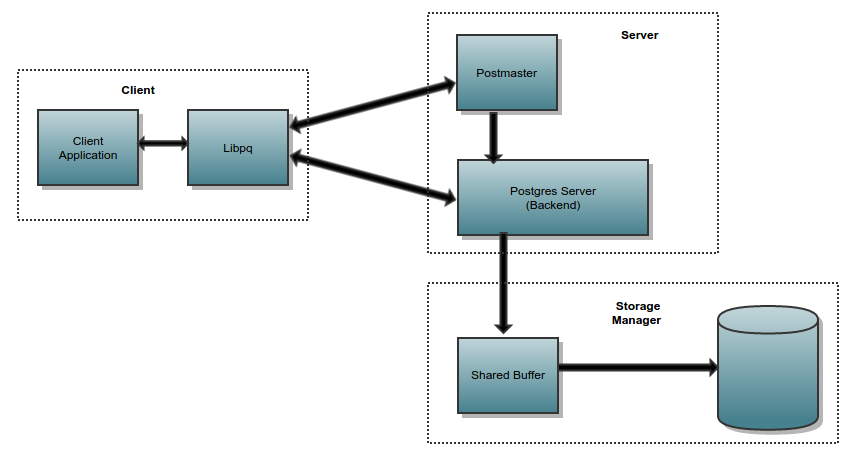
\includegraphics[scale=0.5]{images/arquitecturaPostgresen}}
\caption{PostgreSQL System Concept Architecture \cite{postgresqlpordentro}} \label{fig:ArquitecturaPostgres}
\end{figure}
\subsection{Almacenamiento y organizaci\'on de datos}
Los datos siempre se guardan en el ``disco"  (esto puede no ser literalmente un Hard Drive).
Esto genera un intenso trabajo de I/O(entrada y salida), cuando se lee datos se saca del ``disco'' para pasarla a la memoria RAM, cuando se escribe se baja  de la RAM al ``disco'' como se observa en la Figura \ref{fig:almacenamientoorganizaciondatos}.
\begin{figure}[H]
\centering
\subfigure{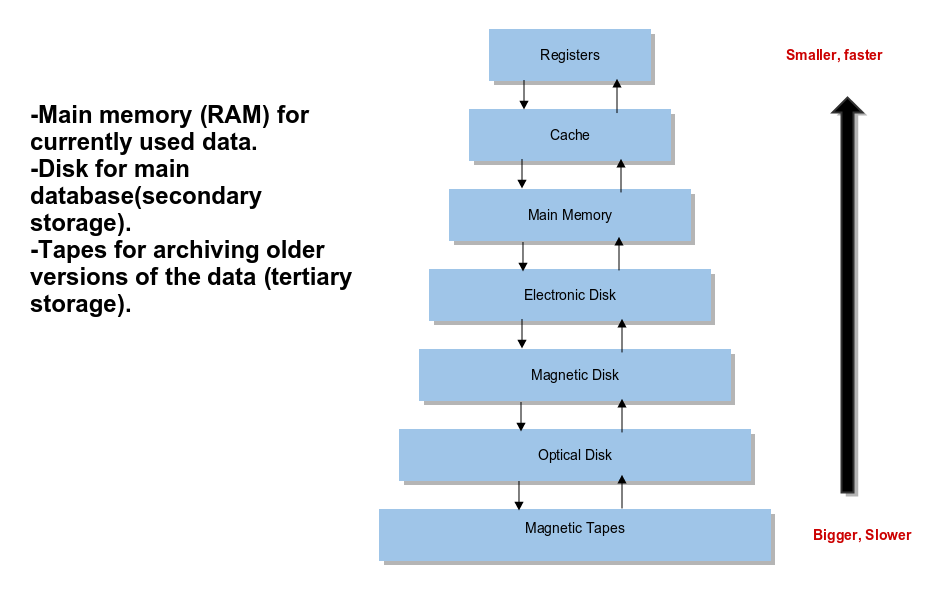
\includegraphics[scale=0.4]{images/almacenamientoorganizaciondatos}}
\caption{Almacenamiento y Organizaci\'on de datos \cite{postgresqlpordentro}} \label{fig:almacenamientoorganizaciondatos}
\end{figure}
PostgreSQL posee un gestor de almacenamiento (Storage Manager) que esta compuesto por varios m\'odulos que proveen administraci\'on de las transacciones y acceso a los objetos de la base de datos.

Los m\'odulos se programaron bajo tres lineamientos bien claros:
\begin{itemize}
\item Manejar transacciones sin necesidad de escribir c\'odigo complejo de recuperaci\'on en caso de ca\'idas.
\item Mantener versiones hist\'oricas  de los datos bajo el concepto de ``graba una vez, lee muchas veces".
\item Tomar las ventajas que ofrece el hardware especializado como multiprocesadores, memoria no vol\'atil.  
\end{itemize}
\subsubsection{Los 'indices}
Cada tipo de b\'usqueda tienen un tipo de \'indice adecuado para trabajarla, b\'asicamente un \'indice es un
 ``archivo" donde est\'a parte de un dato y la estructura de una tabla con  ``search key"  de b\'usqueda.
\subsection{Como se procesa un consulta(Query)}
A continuaci'on se presenta la Figura \ref{fig:comoprocesaquery2} donde se muestra como se procesa una consulta.
\begin{figure}[H]
\centering
\subfigure{\includegraphics[scale=0.25]{images/comoprocesaquery}}
\caption{Como se procesa un query \cite{postgresqlpordentro}} 
\label{fig:comoprocesaquery2}
\end{figure}

Un identificador de reglas de que lo escrito sea sint\'acticamente entendible, que los d\'igitos y los n\'umeros sean reconocibles, luego se descompone ``palabra'' a ``palabra'' el query para pasar a la estructura que le corresponde seg\'un el query, en este caso a la estructura de un \texttt{SELECT}, esto se ve asi:
\lstset{language=sql,breaklines=true}
\label{fig:codigosqlc}
\begin{lstlisting}
simple_select: SELECT opt_distinc target_list
			 into_clause from_clause where_clause
			 group_clause having_clause
			 [
			 	SelectStmt *n = makeNode(SelectStmt);
			 	n->distincClause = $2;
			 	n->targetList = $3;
			 	n->istemp = (bool)((Value *| lfirst($4)))->val.ival;
			 	n->into = (char*) lnext($4);
			 	n->fromClause = $5;
			 	n->whereClause = $6;
				n->groupClause = $7;
				n->havingClause = $8;
				$$ = (Node)n;			 	
			 ]	
\end{lstlisting}

\lstset{language=c,breaklines=true}
\begin{lstlisting}
typedef struct SelectStmt
{
	NodeTag	type;
	List *distincClause;
	
	char *into;
	bool istemp;
	List *targetList;
	List *fromClause;
	Node *whereClause;
	List *groupClause;
	Node *havingClause;
	
	List *sortClause;
	char *portalname;
	bool binary;
	Node *limitOffset;
	Node *limitCount;
	List *forUpdate;
	
	SetOperartion op;
	bool all;
	struct SelectStmt *larg;
	struct SelectStmt *rarg;		
} SelectStmt;	
\end{lstlisting}

\subsubsection{M\'etodos para relacionar tablas}
\subparagraph{Nested loop join}
Consume mas recursos de memoria pero la cantidad de b\'usquedas a realizar es menor.
\subparagraph{Merge join}
Requiere que los datos este ordenada para ubicar las relaciones, el costo esta justamente en mantener la data ordenada.
\subparagraph{Hash join}
Aparentemente ser\'ia la forma mas r\'apida de acceder a un dato gracias a la creaci\'on de tablas indexadas, pero limitada a una b\'usqueda de igualdad. Las combinaciones hash requerir'a una combinaci'on de igualdad predicado (un predicado comparaci'on de los valores de una tabla con los valores de la otra tabla utilizando el operador igual $`='$),las combinaciones hash tambi'en puede ser evaluado por un predicado anti-join (un predicado seleccionar valores de una tabla cuando no hay valores relacionados se encuentran en el otro). Dependiendo de los tama\~nos de las tablas, diferentes algoritmos se pueden aplicar.

El ``Executor" toma el plan de ejecuci\'on que el ``planer" le entrega e inicia el procesamiento, ejecuta un ``plan tree".
Este ``plan tree" tiene varios nodos de ejecuci\'on que se van ejecutando uno a uno y de cada uno de ellos se obtiene un set de datos(tuplas). Los nodos tienen subnodos y otros a su vez otros subnodos, tantos como sea necesario.
\section{Obtener la estructura de una base de datos}
En este caso se requiere obtener una estructura de informaci\'on con detalles por cada columna de una tabla semejante a esta:

\texttt{column\_name} $=>$ \texttt{cedula},
 
\texttt{datatype} $=>$ \texttt{integer}, 

\texttt{key} $=>$ \texttt{PRI},

\texttt{is\_nullable} $=>$ \texttt{NO},

\texttt{max\_length} $=>$ \texttt{8}, 

\texttt{column\_default} $=>$

Se puede observar el detalle de un atributo de una tabla por lo tanto es posible realizar para cada una donde:

\texttt{datatype}: es un tipo de dato interno de postgresql.


key: \texttt{UNI} = \texttt{unique}, el campo es un \'indice \'unico.

 
key:	 \texttt{PRI} = \texttt{primary key}, el campo es un \'indice primario, 

key:	 \texttt{FK} = \texttt{foreign key}, el campo es un \'indice de una llave for\'anea.

max\_length: Si el campo es integer, muestra la precisi\'on del entero (2,4,8), si es un varchar, la longitud en caracteres (ej. 75).

column\_default: muestra el tipo de valor por defecto si la tabla es serial, se puede ver la llamada al nextval de la secuencia: nexval(‘personas\_cliente\_id\_seq'::regclass). Lo que permite determinar que campo de nuestra tabla es serial (auto-incremental).

\subsection{Obtener el detalle de una tabla} 
Para entender cada tabla del \textbf{pg\_catalog}, debe ser interrogada con el \textbf{oid} de la tabla, que se puede obtener de \textbf{pg\_class}.
Los campos y sus atributos se puede sacar de la tabla \textbf{pg\_attribute}.
El tipo de datos se puede sacar de la tabla \textbf{pg\_type}
los constraints de la tabla se obtiene de la tabla \textbf{pg\_constraint}
y el valor por defecto sacar de la tabla \textbf{pg\_attrdef}.
\subsubsection{Usando OIDs}
Los OIDs (Identificador de Objeto) los utiliza PostgreSQL internamente como clave primaria para varias tablas del sistema. Tambi\'en se puede utilizar como identificadores \'unicos en nuestras tablas, aunque es una opci\'on desaconsejable que, a partir de la versi\'on 8.1 viene deshabilitada por defecto en PostgreSQL, por lo tanto no se agregan a las tablas creadas por el usuario, a menos que se especifique \texttt{WITH OIDS} cuando se crea la tabla, o la variable de configuraci\'on \texttt{default\_with\_oids} est\'a habilitada.
A continuaci\'on se presenta el codigo \texttt{SQL} \ref{lst:SQLDetalleTablaMetodoOID} haciendo uso de OIDs.
\begin{lstlisting}[caption={Query para obtener detalle tabla con OIDs},label={lst:SQLDetalleTablaMetodoOID},language=sql]
SELECT pgca.attname as column_name,
	      t.typname as data_type,
CASE
		   WHEN cc.contype='p' THEN 'PRI'
		   WHEN cc.contype='u' THEN 'UNI'
		   WHEN cc.contype='f' THEN 'FK'
		   ELSE '' 
END AS key,	
CASE 
		   WHEN pgca.attnotnull=false THEN 'YES' 
ELSE    'NO' 
END AS is_nullable,
CASE 
		   WHEN pgca.attlen=-1 THEN(pgca.atttypmod-4) 
		   ELSE pgca.attlen 
END as max_length,
d.adsrc as column_default
FROM	 pg_catalog.pg_attribute pgca
		   LEFT JOIN pg_catalog.pg_type t ON
			    t.oid=pgca.atttypid
		   LEFT JOIN pg_catalog.pg_class c ON
			    c.oid=pgca.attrelid
		   LEFT JOIN pg_catalog.pg_constraint cc ON 
			    cc.conrelid=c.oid AND 
			    cc.conkey[1]=pgca.attnum
		   LEFT JOIN pg_catalog.pg_attrdef d ON
			    d.adrelid=c.oid AND 
			    pgca.attnum=d.adnum
WHERE c.relname='nombretabla' AND
	  pgca.attnum>0 AND
	  t.oid = pgca.atttypid.
\end{lstlisting}
\texttt{nombretabla} representa el nombre de la tabla al que se quiere interrogar para obtener su metadato.
Si el modelo de la Figura \ref{fig:Modelo ER} se lleva al gestor de base de datos en este caso PostgreSQL y  se hace uso del c\'odigo de Figura \ref{lst:SQLDetalleTablaMetodoOID} se obtiene algo similar como se observa en la Figura \ref{fig:Detalle Metodo OID} donde:
\begin{itemize}
\item \emph{column\_name} muestra el nombre de la columna de la tabla.
\item \emph{data\_type} indica que tipo almacena esta columna.
\item \emph{key} indica si es una llave, sea primaria, for\'anea o sea \'unico.
\item \emph{is\_nullable} indica si este campo puede ser nulo.
\item \emph{max\_length} indica el tama\~no de memoria de informaci\'on m\'axima.
\item \emph{colum\_default} este campo indica si es autoincremental en PostgreSQL (serial, bigserial y smallserial) que normalmente se suele usar en llaves primarias las cuales no son obligatorias insertar ya que el DBMS se encarga de realizarlo por nosotros.
\end{itemize}
\begin{figure}[H]
\centering
\subfigure{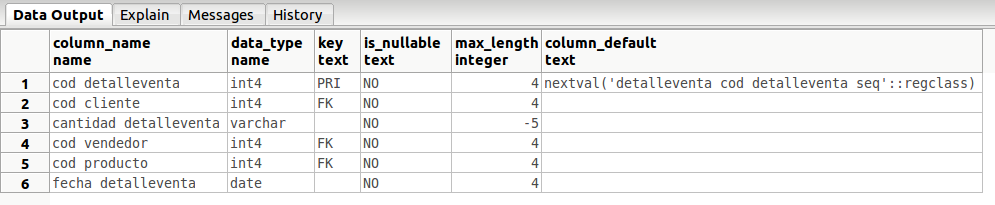
\includegraphics[width=150mm,height=30mm]{images/resDetalleMet1}}
\caption{Detalle tabla OIDs} \label{fig:Detalle Metodo OID}
\end{figure}
Son algunos campos disponibles en el metadato, de las muchas que se puede obtener y depende de lo que sea necesario, las listadas son b\'asicas sobre la informaci\'on detallada de una determina tabla de una base de datos.
\subsubsection{Usando Information schema}
El codigo \ref{lst:SQLDetalleTablaMetodoOID} para obtener los metadatos de una tabla no es la \'unica forma existe otras formas de realizar.
PostgreSQL  a partir de la versi'on 8.0 introdujo el \texttt{INFORMATION\_SCHEMA}. Las vistas definidas en el \texttt{INFORMATION\_SCHEMA} le dan acceso a la informaci'on almacenada en las tablas del sistema PostgreSQL. El \texttt{INFORMATION\_SCHEMA} se define como parte del estandar \texttt{SQL} y encontrar'as un \texttt{INFORMATION\_SCHEMA} en sistemas de bases de datos m'as comerciales (y algunos de c'odigo abierto). Por ejemplo, para ver una lista de las tablas definidas en la base de datos actual, puede ejecutar el c'odigo \ref{lst:SQLDetalleTablaMetodoScheme}:

\begin{lstlisting}[caption={Query para detalle obtener el detalle de una tabla information scheme},label={lst:SQLDetalleTablaMetodoScheme},language=sql]
SELECT tc.column_name,
       data_type,
       character_maximum_length,
       numeric_precision,
       is_nullable,
       tcs.constraint_type,
       column_default,
       check_clause
FROM information_schema.columns AS tc
     LEFT OUTER JOIN
        information_schema.constraint_column_usage AS cc
     	ON tc.table_name = cc.table_name AND
        tc.column_name = cc.column_name
     LEFT OUTER JOIN
        information_schema.table_constraints AS tcs
     	ON tcs.constraint_name = cc.constraint_name
     LEFT OUTER JOIN
        information_schema.check_constraints AS cccs
     	ON cccs.constraint_name = tcs.constraint_name
WHERE tc.table_name = 'NOMBRE DE LA TABLA' AND
      tc.table_schema = 'public' AND
     (tcs.constraint_type='PRIMARY KEY' OR 
      tcs.constraint_type='CHECK' OR 
      tcs.constraint_type ISNULL)
ORDER BY ordinal_position;
\end{lstlisting}
Si se hace una comparaci'on con la anterior se puede ver las diferencias, en esta ya no se hace uso de los \texttt{OIDS} las tablas que son parte del metadato, las tablas necesarias para esta consulta son:

\lstset{language=sql,breaklines=true}
\begin{lstlisting}
SELECT * FROM information_schema.columns
SELECT * FROM information_schema.constraint_column_usage
SELECT * FROM information_schema.table_constraints
SELECT * FROM information_schema.check_constraints
\end{lstlisting}
Si se ejecuta el codigo \ref{lst:SQLDetalleTablaMetodoScheme} se obtiene como resultado lo que se ve en la Figura \ref{fig:DetalleMetodoScheme}.

\begin{figure}[H]
\centering
\subfigure{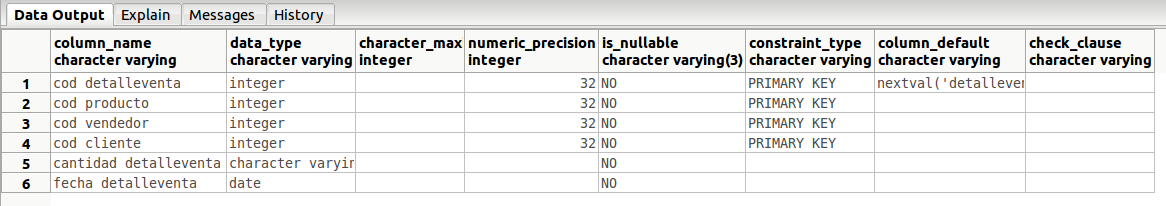
\includegraphics[width=150mm,height=30mm]{images/resDetalleMet2}}
\caption{Information schema} \label{fig:DetalleMetodoScheme}
\end{figure}
Donde se puede hacer una descripcion detallada:
\begin{itemize}
\item \emph{column\_name} muestra el nombre de la columna de la tabla.
\item \emph{data\_type} indica el tipo de datos que esta permitido insertar, si se compara con los resultados de la figura \ref{fig:Detalle Metodo OID} aqu\'i devuelve el tipo de dato (integer en lugar de int4) como se definio en el modelo de la Figura \ref{fig:Modelo ER} Modelo ER.
\item \emph{constraint\_type} indica si es una llave sea primaria, for\'anea o sea \'unico.
\item \emph{is\_nullable} indica si este campo puede ser nulo.
\item \emph{character\_max\_length} indica el tama\~no de memoria de informaci\'on m\'axima.
\item \emph{colum\_default} en este campo indica si es autoincrementable en PostgreSQL(serial, bigserial y smallserial) que normalmente se suele usar en llaves primarias las cuales no son obligatorias insertar ya que el DBMS se encarga de realizarlo.
\item \emph{check\_clause} en esta columna se muestra si el campo tiene restricciones al realizar la inserci\'on de datos por ejemplo: se puede decidir si se quiere registrar edades entre 18 a 60 a\~nos. 
\item \emph{numeric precision} indica el tama\~no del tipo, aparte de pertenecer a un cierto tipo en los DBMS suelen tener tipos de datos mas precisos.  
\end{itemize}
\subsection{Obteniendo las relaciones entre las tablas}
La estructura de las relaciones entre tablas en una base de datos es el resultado de su modelo ER, donde las relaciones en PostgreSQL son representadas por \textit{constraints} en un sistema gestor de base de datos.
De alguna manera se necesita saber mediante un script las relaciones entre tablas de una base de datos, que tablas se relacionan con otra y exactamente que columnas est\'an involucradas, al decir las columnas involucradas se menciona exactamente a las columnas de una determinada tabla que son las llaves for\'aneas y que estas existen en la tabla que es referenciada, si se ejecuta el c'odigo \ref{SQL Tablas que referencian}.
\begin{lstlisting}[caption={Query para obtener el detalle de referencias},label={SQL Tablas que referencian},language=sql]
SELECT (SELECT relname
        FROM pg_catalog.pg_class c
        	LEFT JOIN pg_catalog.pg_namespace n ON
		       n.oid = c.relnamespace
        WHERE c.oid=r.conrelid) as tablas,
        conname,
        pg_catalog.pg_get_constraintdef(oid, true) as ref 
FROM pg_catalog.pg_constraint r 
WHERE r.conrelid 
	  IN(SELECT c.oid 
		    FROM pg_catalog.pg_class c LEFT JOIN
           pg_catalog.pg_namespace n ON 
		         n.oid = c.relnamespace 
      WHERE c.relname !~ 'pg_' AND 
            c.relkind = 'r' AND 
            pg_catalog.pg_table_is_visible(c.oid)) AND 
r.contype = 'f'
\end{lstlisting}
 Se tiene el resultado como se observa en la Figura \ref{fig:Referencias entre tablas}.
\begin{figure}[H]
\centering
\subfigure{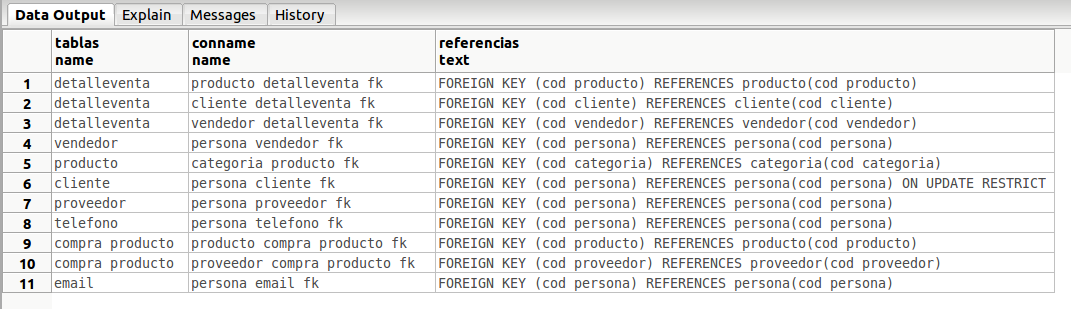
\includegraphics[width=150mm,height=45mm]{images/resReferencias}}
\caption{Referencias entre tablas} \label{fig:Referencias entre tablas}
\end{figure}
A continuaci'on se puede ver un detalle:
\begin{itemize}
\item \textbf{tablas} Muestra la lista de tablas que hacen referencia, puede encontrarse que el nombre de una tabla llegue a repetirse en mas de una ocasi\'on no es un problema, se hara un detalle despu\'es de ver la explicaci\'on de la tercera columna.   
\item \textbf{conname} Muestra el \texttt{CONSTRAINT} de la relaci\'on, que seria algo como el nombre de la relaci\'on entre las tablas involucradas. 
\item \textbf{referencias} En esta columna de la Figura \ref{fig:Referencias entre tablas} trae toda la informaci\'on necesaria para ser usado. se puede ver la cadena de texto de una de ellas:
\lstset{language=sql,breaklines=true}
\begin{lstlisting}
"FOREIGN KEY (cod_producto) REFERENCES producto(cod_producto)"
\end{lstlisting}
La cadena de texto posee informaci\'on relevante donde \emph{(cod\_producto)} es el campo que hace referencia como indica \texttt{REFERENCES} a la tabla \emph{producto} y al campo  \emph{(cod\_producto)}.
Aunque el resultado esta en modo texto existen formas de solucionar para obtener la informaci\'on separada, una manera es realizar un parseo al texto que las distintos lenguajes de programaci\'on ya tienen funciones implementadas para estas tareas. 
\end{itemize}
En la columna \emph{tablas} llegan a repetirse el nombre de una tabla en mas de una vez, esto es debido a que lista por cada relaci\'on que llegue a tener una tabla con otras
\subsection{Obteniendo las tablas independientes}
Para obtener las tablas que son independientes de otras es necesario usar el script anterior la cual da como resultado un conjunto solo de las tablas que se relacionan de alguna manera entre ellas y tener otro conjunto de todas las tablas de la base de datos, como se tiene estos dos conjuntos de tablas realizar una operaci\'on de resta entre los conjuntos. La lista de todas las tablas menos la lista de las tablas que se relacionan, como resultado se tiene las tablas que son independientes y que llegar\'ian a ser los primeros en ser llenados.
El c\'odigo \texttt{SQL} para obtener esa informaci\'on es la que se tiene en el c'odigo \ref{SQL Tablas independientes}.
\begin{lstlisting}[caption={Query para obtener tablas independientes},label={SQL Tablas independientes},language=sql]
SELECT tablename
FROM pg_tables
WHERE schemaname = 'public' AND
      tablename NOT IN
     (SELECT (SELECT relname 
      		      FROM pg_catalog.pg_class c LEFT JOIN
                   pg_catalog.pg_namespace n ON 
                   n.oid = c.relnamespace 
              WHERE
                   c.oid=r.conrelid) as nombre
      FROM pg_catalog.pg_constraint r 
      WHERE r.conrelid IN
            (SELECT c.oid
             FROM pg_catalog.pg_class c LEFT JOIN
                  pg_catalog.pg_namespace n ON 
                  n.oid = c.relnamespace 
             WHERE c.relname !~ 'pg_' AND 
                   c.relkind = 'r' AND 
                   pg_catalog.pg_table_is_visible(c.oid))
      AND r.contype = 'f')
\end{lstlisting}
Si se ejecuta esta consulta da como resultado como se observa en la Figura \ref{fig:Tablas independientes}.

Al analizar la Figura \ref{fig:Modelo ER} Modelo ER se puede observar que las entidades que son independientes que no hacen referencia a otra son las mismas que da como resultado en la Figura \ref{fig:Tablas independientes}.
\begin{figure}[H]
\centering
\subfigure{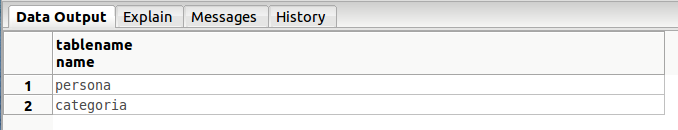
\includegraphics[width=150mm,height=30mm]{images/resTablasInd}}
\caption{Tablas independientes} \label{fig:Tablas independientes}
\end{figure}
\section{Ordenando los metadatos}
Si ya se cuenta con la informaci\'on de los metadatos de una base de datos es necesario por una parte tener claro en el detalle de una tabla, que las llaves for\'aneas pueden ser un conjunto de columnas que hagan referencia a una determinada tabla.

Al momento de hacer las inserciones de datos se debe tener cuidado con este caso si se inserta valores a columnas que hacen referencia estas deben existir en la tabla referenciada.

Como se puede observar en la Figura \ref{fig:ModeloERcomp} la entidad venta es una composici\'on de \textit{vendedor} y \textit{cliente} y que esta a la vez llega ser maestra de la entidad \textit{detalle}, por lo tanto la entidad \textit{detalle} tiene una llave compuesta.
\begin{figure}[H]
\centering
\subfigure{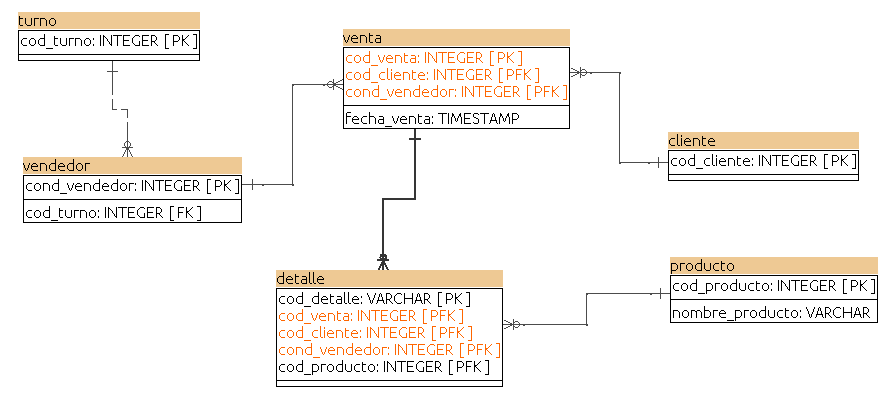
\includegraphics[scale=0.5]{images/ModeloERcomp}}
\caption{Modelo ER compuesto} \label{fig:ModeloERcomp}
\end{figure}
Si el modelo se lleva a un sistema gestor de base de datos en este caso PostgreSQL y se llena con datos de prueba como se ve en la Figura \ref{fig:tabla venta} se tiene  llaves compuestas.
\begin{figure}[H]
\centering
\subfigure{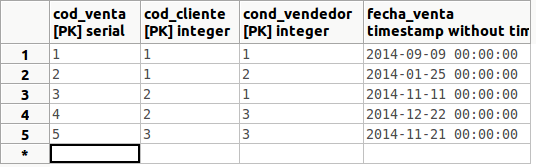
\includegraphics[width=130mm,height=40mm]{images/tablaVenta}}
\caption{Tabla venta} \label{fig:tabla venta}
\end{figure}

Al realizar la inserci\'on en \textit{detalle} se debe tener cuidado en no cometer el error de la ultima inserci\'on que se quiere hacer en la Figura \ref{fig:InsercionIncorrecta}, esta llega a ser incorrecta debido a que no existe una fila de (\textit{cod\_venta,cod\_cliente,cod\_vendedor}) en la tabla \textit{venta} con valores de (\textit{2,1,1}), llegando a no cumplir la integridad referencial adem\'as son datos inconsistentes. 

La ultima inserci'on de la Figura \ref{fig:InsercionCorrecta} es correcta porque en la Figura \ref{fig:tabla venta} se puede encontrar una fila tambi\'en conocida como tupla que (\textit{cod\_venta,cod\_cliente,cod\_vendedor}) tengan los valores (\textit{2,1,2}) cumpliendo as\'i la integridad referencial y consistencia de datos.

\begin{figure}[H]
\centering
\subfigure{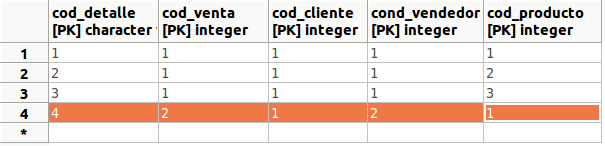
\includegraphics[width=130mm,height=35mm]{images/tablaDetalleCorrecto}}
\caption{Tabla detalle inserci'on correcta} \label{fig:InsercionCorrecta}
\end{figure}

\begin{figure}[H]
\centering
\subfigure{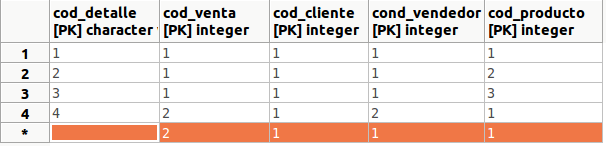
\includegraphics[width=130mm,height=35mm]{images/tablaDetalleIncorrecto}}
\caption{Tabla detalle inserci'on incorrecta} \label{fig:InsercionIncorrecta}
\end{figure}  
  
La otra parte es ordenar la lista de tablas seg\'un la prioridad que deben ser llenados, esta claro que las tablas independientes son los primeros de ahi en adelante aun no esta claro, por lo tanto es necesario desarrollar mecanismos para obtener una lista de tablas seg\'un el orden en que se requiere.
\subsection{Ordenando las tablas}
El codigo \ref{SQL Tablas independientes} da  como resultado las tablas que deben ser llenados primero, las siguientes son algunas de la lista que entrega el codigo \ref{SQL Tablas que referencian}, que pr\'acticamente est\'an desordenados.

Si el modelo entidad relaci\'on de la Figura \ref{fig:ModeloERcomp} se lleva a postgreSQL y se aplica el codigo \ref{SQL Tablas que referencian} se obtiene el resultado de la Figura \ref{fig:referenciasModeloComp}

\begin{figure}[H]
\centering
\subfigure{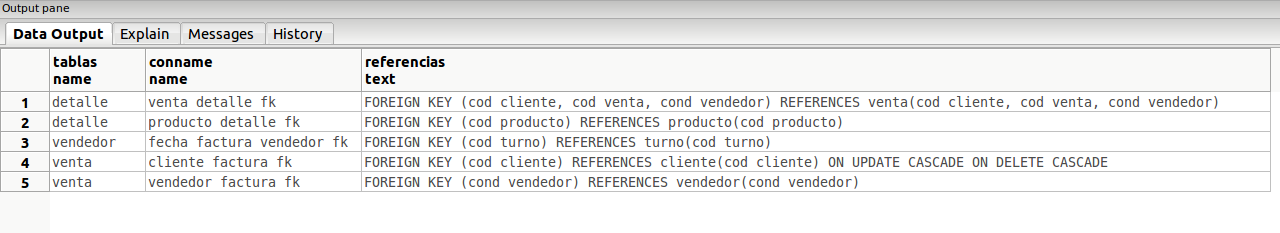
\includegraphics[scale=0.36]{images/referenciasModeloComp}}
\caption{Detalle de relaciones entre tablas} \label{fig:referenciasModeloComp}
\end{figure}

En la Figura \ref{fig:referenciasModeloComp} se tiene la primera columna el nombre de la tabla que hace referencia a una o mas tablas, pero en la tercera columna no se tiene separada el nombre de la tabla que es referenciada por que es necesario separarlos de alguna manera, el formato de texto que da como resultado para la primera linea perteneciente a \textit{detalle}:
\lstset{language=sql,breaklines=true}
\begin{lstlisting}
"FOREIGN KEY (cod_cliente, cod_venta, cond_vendedor) REFERENCES venta(cod_cliente, cod_venta, cond_vendedor)"
\end{lstlisting}
Lo que hace es separar en cinco partes la cadena de texto:
\begin{enumerate}
\item \texttt{FOREIGN KEY}
\item \texttt{cod\_cliente, cod\_venta, cond\_vendedor}
\item \texttt{REFERENCES venta}
\item \texttt{cod\_cliente, cod\_venta, cond\_vendedor}
\item ...
\end{enumerate}
Las manera de implementar puede variar de acuerdo a la tecnolog\'ia sea java, php, python y otros, sin embargo muchas de estas tecnolog\'ias ya vienen implementadas estas funciones para hacer estas tareas, por ejemplo en java se puede llevar la cadena de texto a un arreglo de textos simplemente se define delimitadores que este caso serian $`` (  ,  )  "$   obteniendo as\'i un resultado similar a la que se listo. A partir de esa lista se escoge el de la posici\'on 2 iniciando a contar desde 0 que llega ser \textit{REFERENCES venta} en este caso en particular, esta cadena se vuelve a separar en dos:
\begin{enumerate}
\item \texttt{REFERENCES}
\item \texttt{venta}
\end{enumerate}
Como se tiene el nombre de la tabla se retorna este valor como la tabla que es referenciada para \textit{detalle}. Se realiza esto para cada una de la lista de la Figura \ref{fig:referenciasModeloComp}.

Cabe aclarar que en la segunda columna en la segunda separaci\'on de texto que se hizo puede que en algunos casos sobre todo cuando se hace uso de scheme(esquemas) en postgreSQL venga concatenada el nombre del scheme antes del nombre de la tabla concatenada con un punto seguido con el nombre de la tabla.

\texttt{public.venta.}

Lo cual no deber\'ia  causar problemas por el simple hecho de que ayuda a identificar en que scheme se encuentra la tabla. Como resultado de las operaciones que se hizo se obtiene el resultado que se observa en el cuadro \ref{table3}.
\begin{center}
\scriptsize
  \captionof{table}{tablas que referencian a otra}
  \renewcommand{\arrayrulewidth}{1pt}
  \label{table3} % for use in \ref{table1} if you want to refer to the table number
\begin{tabular}{|p{40mm}|p{98mm}|}
\hline
\textbf{tablas que referencian} & \textbf{tablas referenciadas} \\ \hline
detalle                         & venta                         \\ \hline
detalle                         & producto                      \\ \hline
vendedor                        & turno                         \\ \hline
venta                        & cliente                       \\ \hline
venta                           & vendedor                      \\ \hline
\end{tabular}
\end{center}
En la primera columna se tiene las tablas que hacen referencia y en la segunda columna las que son referenciados. Para hacer uso del algoritmo de ordenaci\'on \ref{Algoritmo de ordenamiento} del Capitulo \ref{Algoritmos de ordenamiento y mecanismos del manejo referencial},  ya se cuenta con datos hasta el paso dos por lo tanto pasar al paso tres donde se realiza la b'usqueda para todas aquellas entidades que le hacen referencia a los que son independientes, que para el modelo ER de la Figura \ref{fig:ModeloERcomp} llegar\'ia a ser la figura \ref{desodenadocomp}.
\begin{figure}[H]
\centering
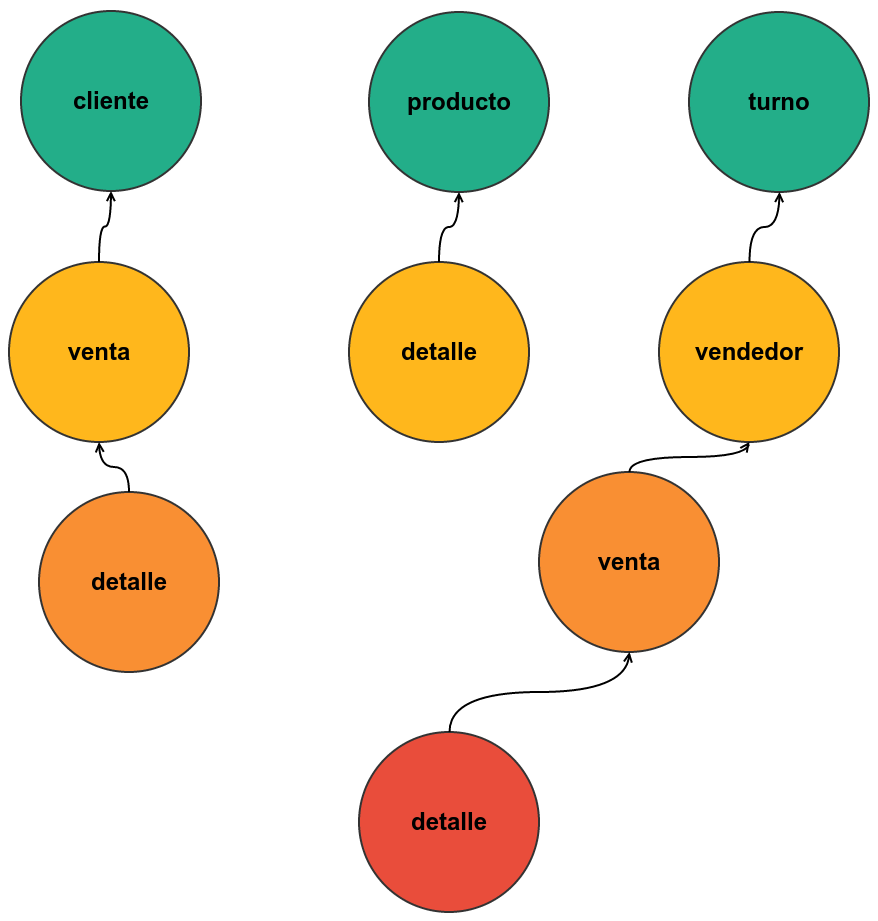
\includegraphics[scale=0.2]{images/desordenadocomp.png}
\caption{Secuencia}
\label{desodenadocomp}
\end{figure}
Donde se puede observar que el nombre de una tabla se llega a repetir en varios lugares para lo cual se aplica el \ref{Algoritmo de ordenacion primeros en ser llenado} de Capitulo \ref{Algoritmos de ordenamiento y mecanismos del manejo referencial} , como resultado se llega a tener la figura \ref{ordencorrectonodos} la cual tiene el orden correcto.
\begin{figure}[H]
 \centering
 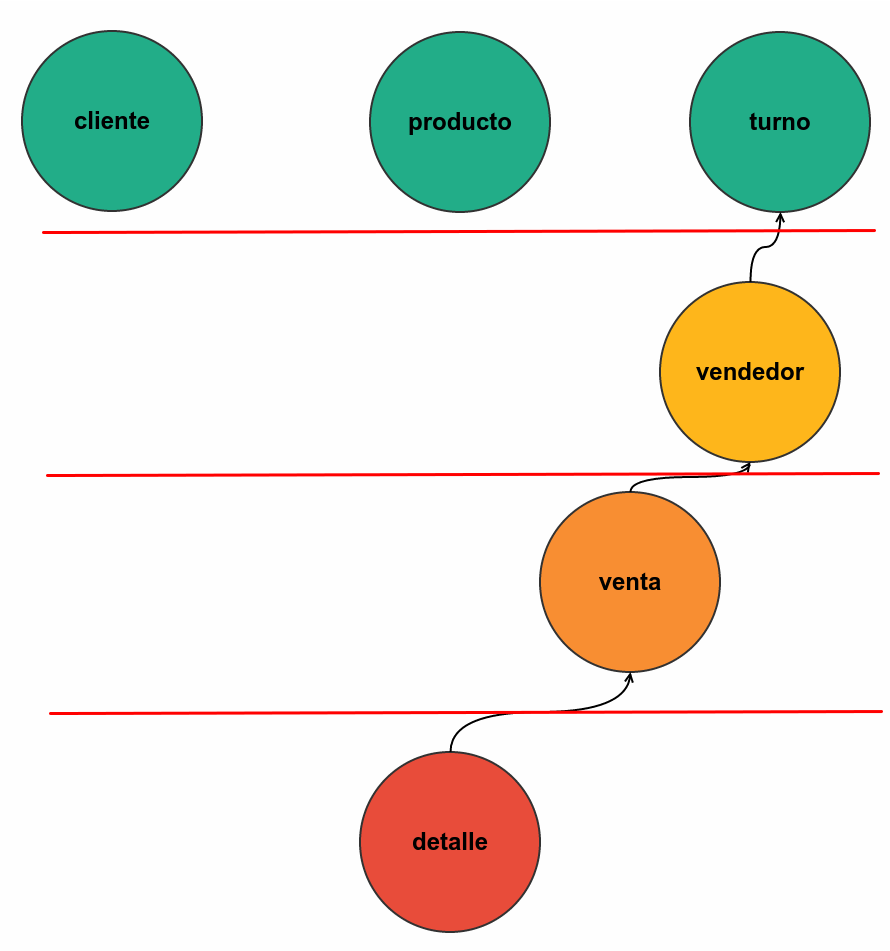
\includegraphics[scale=0.2]{images/ordenadocomp.png}
 \caption{Orden correcto}
 \label{ordencorrectonodos}
 \end{figure}
  
\subsection{Uniendo \texttt{foreign keys}}
Una vez que ya se tiene la informaci\'on detallada por cada una de las tablas que hacen referencia y de las cuales las columnas que est\'en involucradas llegan a ser llaves extranjeras, que si bien pueden ser parte de la llave primaria compuesta de la tabla o simplemente ser una llave for\'anea, al momento de insertar puede llegar a dar lo mismo, por lo tanto no se va a centrar en ese detalle.

La informaci\'on que provee el query de la Figura \ref{lst:SQLDetalleTablaMetodoScheme} da una detallada informaci\'on sobre una tabla en particular pero para lo que se necesita generar datos de prueba es importante tener mecanismos que eviten cometer errores en las llaves que no son propias de una tabla. En el query de la Figura \ref{fig:referenciasModeloComp} se tiene una informaci\'on valiosa en la tercera columna:

\lstset{language=sql,breaklines=true}
\begin{lstlisting}
"detalle";"venta_detalle_fk";"FOREIGN KEY (cod_cliente, cod_venta, cond_vendedor) REFERENCES venta(cod_cliente, cod_venta, cond_vendedor)"
"detalle";"producto_detalle_fk";"FOREIGN KEY (cod_producto) REFERENCES producto(cod_producto)"
\end{lstlisting}
La tabla \textit{detalle} con las columnas \textit{(cod\_cliente, cod\_venta, cond\_vendedor)} hace referencia a la tabla \textit{venta} a las columnas \textit{(cod\_cliente, cod\_venta, cond\_vendedor)}, adem\'as la columna \textit{(cod\_producto)} hace referencia a la tabla \textit{producto} a la columna \textit{(cod\_producto)}, son las llaves que no son propias de la tabla \textit{detalle}.

En el detalle que da como informaci\'on la Figura \ref{fig:detalleTablaDetalle},  las llaves que no son propias no est\'an agrupadas de acuerdo a la tabla al que referencia como sucede en la Figura \ref{fig:referenciasModeloComp} donde si lo agrupa pero solo provee esos campos que son llaves que apuntan a otra tabla, a diferencia de la Figura \ref{fig:detalleTablaDetalle} si da la informaci\'on de todas las columnas.

\begin{figure}[H]
\centering
\subfigure{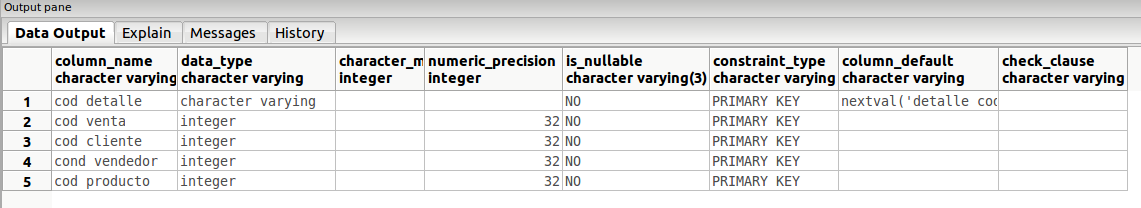
\includegraphics[width=150mm,height=35mm]{images/detalleTablaDetalle}}
\caption{Detalle de la tabla \textit{detalle}} \label{fig:detalleTablaDetalle}
\end{figure}
El cuadro \ref{tableReferenciasTablaDetalle1} es resultado al que se quiere llegar uniendo la informaci\'on de la Figura \ref{fig:detalleTablaDetalle} y la Figura \ref{fig:detalleTablaDetalle}.

\begin{center}
\scriptsize
  \captionof{table}{tabla de referencias para la tabla detalle}
\renewcommand{\arrayrulewidth}{1pt}  
  \label{tableReferenciasTablaDetalle1} % for use in \ref{table1} if you want to refer to the table number
  \begin{tabular}{|l|p{10mm}|p{45mm}|l|l|l|}
\hline
\textbf{\begin{tabular}[c]{@{}l@{}}nombre\\ columna\end{tabular}}                   & \textbf{\begin{tabular}[c]{@{}l@{}}tipo\\ de\\ dato\end{tabular}} & \textbf{es primaria?} & \textbf{serial} & \textbf{\begin{tabular}[c]{@{}l@{}}tabla a\\ la que\\ referencia\end{tabular}} & \textbf{\begin{tabular}[c]{@{}l@{}}columnas a la\\ que referencia\end{tabular}}     \\ \hline
cod\_detalle                                                                        & \texttt{INTEGER}                                                         & \texttt{PRIMARY KEY}  & si              & \texttt{NULL}                                                                         & null                                                                                \\ \hline
cod\_producto                                                                       &                                                                 & FORANEA               &                 & producto                                                                     & cod\_producto                                                                       \\ \hline
\begin{tabular}[c]{@{}l@{}}cod\_venta,\\ cod\_cliente,\\ cod\_vendedor\end{tabular} &                                                                 & FORANEA               &                 & venta                                                                        & \begin{tabular}[c]{@{}l@{}}cod\_venta,\\ cod\_cliente,\\ cod\_vendedor\end{tabular} \\ \hline
\end{tabular}
\end{center}
Si se recuerda el query de la Figura \ref{SQL Tablas que referencian} da como resultado una lista de tablas que referencian, en este caso solo es necesario consultar especificamnete para una tabla, para lo cual se hace alguna modificaci\'on a la consulta del c'odigo \ref{SQL Tablas que referencian} quedando como  resultado el c'odigo \ref{muestra detalle tabla por tabla}.

\begin{lstlisting}[caption={Query para detalle referencias para una tabla},label={muestra detalle tabla por tabla},language=sql]
SELECT(SELECT relname
       FROM pg_catalog.pg_class c 
            LEFT JOIN 
                 pg_catalog.pg_namespace n ON 
                 n.oid=c.relnamespace
       WHERE
            c.oid=r.conrelid) as nombre,
       conname,
       pg_catalog.pg_get_constraintdef(oid,true)AS ref 
FROM
        pg_catalog.pg_constraint r 
WHERE r.conrelid IN
        (SELECT 
                c.oid 
         FROM pg_catalog.pg_class c 
             LEFT JOIN
                pg_catalog.pg_namespace n ON 
                n.oid = c.relnamespace 
         WHERE 
               c.relname !~ 'pg_' AND 
               c.relkind='r' AND 
               pg_catalog.pg_table_is_visible(c.oid))AND
      r.contype = 'f' AND 
        (SELECT relname 
         FROM pg_catalog.pg_class c 
             LEFT JOIN
              pg_catalog.pg_namespace n ON
              n.oid = c.relnamespace 
         WHERE
              c.oid=r.conrelid)='nombreTabla';";
\end{lstlisting}
A diferencia de la consulta del c'odigo \ref{SQL Tablas que referencian} en esta consulta se especifica exactamente para que tabla se quiere saber a quienes referencia agregando al final las siguientes lineas de c\'odigo \texttt{SQL} \ref{muestra detalle tabla por tabla plus}.

\begin{lstlisting}[caption={Parte que determina para una tabla},label={muestra detalle tabla por tabla plus},language=sql]
           AND 
            (SELECT relname 
             FROM pg_catalog.pg_class c 
                  LEFT JOIN
                  pg_catalog.pg_namespace n ON
                  n.oid = c.relnamespace 
             WHERE
                   c.oid=r.conrelid)='nombreTabla';";
\end{lstlisting}
Con la adici'on del c'odigo extra se logra que filtre solo para la tabla que se requiere, bastara con solo cambiar el \textit{nombreTabla}.
El resultado de esta consulta  dar\'ia solo los registros donde una determinada tabla hace referencia, ver para el caso de la tabla \textit{detalle} en la Figura \ref{fig:referenciasTablaDetalle}.

\begin{figure}[H]
\centering
\subfigure{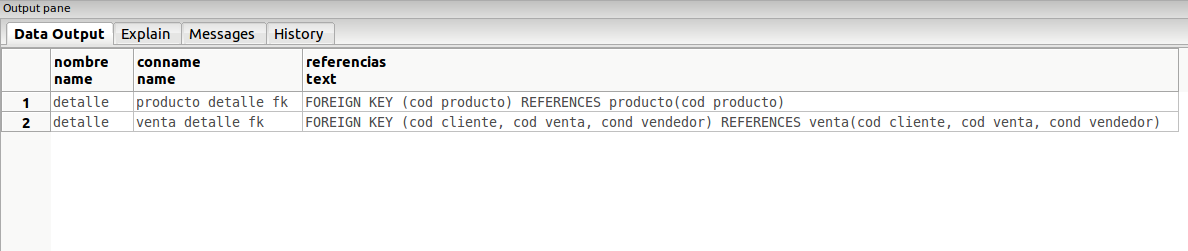
\includegraphics[width=150mm,height=40mm]{images/referenciasTablaDetalle}}
\caption{Detalle de referencias de la tabla detalle} \label{fig:referenciasTablaDetalle}
\end{figure}

Los resultados no llegan a ser tan buenos debido a que devuelve en texto todo los datos de las columnas que referencian y la tabla que es referenciada con sus respectivos columnas. Se har'a uso de las mismas t'ecnicas que se aplico al momento de realizar el ordenamiento de las tablas seg'un el orden que deben ser llenados que al final se necesita tener un resultado similar al cuadro \ref{tablaReferenciasFormateada1}.

\begin{center}
\scriptsize
  \captionof{table}{tabla referencias formateada}
  \label{tablaReferenciasFormateada1} % for use in \ref{table1} if you want to refer to the table number
  \begin{tabular}{|l|l|l|l|}
\hline
\textbf{\begin{tabular}[c]{@{}l@{}}tabla que \\ referencia\end{tabular}} & \textbf{\begin{tabular}[c]{@{}l@{}}columnas que \\ referencian\end{tabular}}           & \textbf{\begin{tabular}[c]{@{}l@{}}tabla \\ referenciada\end{tabular}} & \textbf{\begin{tabular}[c]{@{}l@{}}columnas \\ referenciadas\end{tabular}} \\ \hline
detalle                                                                  & cod\_producto                                                                          & producto                                                               & cod\_producto                                                              \\ \hline
detalle                                                                  & \begin{tabular}[c]{@{}l@{}}cod\_cliente, \\ cod\_venta,\\  cond\_vendedor\end{tabular} & venta                                                                  & cod\_cliente, cod\_venta, cond\_vendedor                                   \\ \hline
\end{tabular}
\end{center}

De la Figura \ref{fig:referenciasTablaDetalle} se toma la columna 3 y la fila 2 como ejemplo escoger la fila 2 por razones did'acticas, es donde se encuentra la informaci\'on en modo texto:
\lstset{language=sql,breaklines=true}
\begin{lstlisting}
"FOREIGN KEY (cod_cliente, cod_venta, cond_vendedor) REFERENCES venta(cod_cliente, cod_venta, cond_vendedor)"
\end{lstlisting}
 La cadena de texto se separa en 5 partes:
 
 \textit{Lista en 5 partes}
 \begin{enumerate}
 \item \texttt{FOREIGN KEY}
 \item \texttt{cod\_cliente, cod\_venta, cond\_vendedor}
 \item \texttt{REFERENCES venta}
 \item x\texttt{REFERENCES venta}
 \item ...
 \end{enumerate}
 
 Para obtener esta lista separada se lleva a un arreglo la cadena de texto teniendo como separadores a ``,''. La mayor'ia de los lenguajes de programaci\'on proveen funciones que realizan esta tarea de llevar una cadena de texto a un arreglo con solo indicar los caracteres separadores.
 
 En la mayor'ia de los lenguajes de programaci'on el conteo de las posiciones se inicia en 0 por tanto es necesario basarse en esa regla, del arreglo solo se necesita el de la posici'on 1, que se encuentra las columnas que hacen referencia en conjunto a la tabla de la posici'on 2 de arreglo, sin antes aclarar que este elemento de la posici'on debe ser separado en dos partes:
 
\textit{} 
 \begin{enumerate}
 \item \texttt{REFERENCES}
 \item venta.
\end{enumerate}  

Entre \texttt{REFERENCES} y \texttt{venta} solo es necesario \texttt{venta} que llega a ser el nombre de la tabla referenciada.

Si se vuelve a la lista separada en 5 partes el otro elemento 'util es de la posici'on 3, es donde se encontro las columnas referenciadas.

Se realiza este procedimiento por cada relaci'on que haga la tabla obteniendo as'i un resultado similar a la tabla del cuadro \ref{tablaReferenciasFormateada1}.
Con los resultados obtenidos de la Figura \ref{fig:detalleTablaDetalle} y el de la Figura tabla formateada del cuadro \ref{tablaReferenciasFormateada1} realizar la union de estos dos resultados para tener una tabla como se ve en el cuadro \ref{tableReferenciasTablaDetalle1}.

Para obtener un resultado del cuadro \ref{tableReferenciasTablaDetalle1} es necesario agregar campos al resultado que provee la Figura \ref{fig:detalleTablaDetalle}, agregar cuatro campos adicionales:
\begin{itemize}
	\item \textit{es\_foranea} En esta columna se puede agregar si es for'anea o no para luego ser evaluado como tal.
	\item \textit{referencian} En esta columna agregar los nombres de las columnas que hacen referencia a otra tabla.
	\item \textit{tabla} En esta columna agregar el nombre de la tabla al que referencia.
	\item \textit{referenciados} En esta columna agregar los nombres de las columnas que son referenciados.
\end{itemize}
Quedando como resultado el cuadro \ref{tablaDetalleAumentadaColumnas1}.

\begin{center}
\scriptsize
  \captionof{table}{tabla con columnas aumentadas para la tabla \textit{detalle}}
  \label{tablaDetalleAumentadaColumnas1} % for use in \ref{table1} if you want to refer to the table number
  \begin{tabular}{|l|l|l|l|l|l|l|l|}
\hline
column\_name  & data\_type                                                  & constraint\_type & .......... & es\_foranea & \begin{tabular}[c]{@{}l@{}}columnas\\ referencian\end{tabular} & \begin{tabular}[c]{@{}l@{}}tabla\\ referenciada\end{tabular} & \begin{tabular}[c]{@{}l@{}}columnas\\ referenciadas\end{tabular} \\ \hline
cod\_detalle  & \begin{tabular}[c]{@{}l@{}}character\\ varying\end{tabular} & PRIMARY\_KEY     & .........  &             &                                                                &                                                              &                                                                  \\ \hline
cod\_venta    & \texttt{INTEGER}                                                    & \texttt{PRIMARY\_KEY}     &            &             &                                                                &                                                              &                                                                  \\ \hline
cod\_cliente  & \texttt{INTEGER}                                                     & \texttt{PRIMARY\_KEY}    &            &             &                                                                &                                                              &                                                                  \\ \hline
cod\_vendedor & \texttt{INTEGER}                                                     & \texttt{PRIMARY\_KEY}     &            &             &                                                                &                                                              &                                                                  \\ \hline
cod\_producto & \texttt{INTEGER}                                                     & \texttt{PRIMARY\_KEY}     &            &             &                                                                &                                                              &                                                                  \\ \hline
\end{tabular}
\end{center}

Si se recuerda la cadena de texto: 
\lstset{language=sql,breaklines=true}
\begin{lstlisting}
"FOREIGN KEY (cod_cliente, cod_venta, cond_vendedor) REFERENCES venta(cod_cliente, cod_venta, cond_vendedor)
FOREIGN KEY (cod_producto) REFERENCES producto(cod_producto)"
\end{lstlisting}
Se lleva a un arreglo de 5 elementos, el elemento de la posici'on 1 que llega a ser lo siguiente:
\lstset{language=sql,breaklines=true}
\begin{lstlisting}
"cod_cliente, cod_venta, cond_vendedor"
\end{lstlisting}
Es donde se encuentra las columnas que hacen referencia por lo tanto a esta cadena es necesario tambi'en llevar a un arreglo lineal donde el car'acter separador llega a ser el $`` , " $  quedando como resultado  el cuadro \ref{columnasQueRefencian1}.
\begin{center}
\scriptsize
\renewcommand{\arrayrulewidth}{1pt}
  \captionof{table}{columnas de la tabla detalle que referencian a venta}
  \label{columnasQueRefencian1} % for use in \ref{table1} if you want to refer to the table number
  \begin{tabular}{|l|l|l|l|}
\hline
\textbf{nombre columna} & cod\_cliente & cod\_venta & cond\_vendedor \\ \hline
\textbf{posicion}       & 0            & 1          & 2              \\ \hline
\end{tabular}
\end{center}


\begin{center}
\scriptsize
\renewcommand{\arrayrulewidth}{1pt}
  \captionof{table}{columna de la tabla detalle que referencia a producto}
  \label{columnaQueRefencian2} % for use in \ref{table1} if you want to refer to the table number
  \begin{tabular}{|l|l|}
\hline
\textbf{nombre columna} & cod\_producto \\ \hline
\textbf{posici'on}      & 0             \\ \hline
\end{tabular}
\end{center}

Los datos del cuadro \ref{columnasQueRefencian1} y \ref{columnaQueRefencian2} son las que hacen referencia a otra tabla para unir las llaves for'aneas y llegar a un resultado como en el cuadro \ref{tableReferenciasTablaDetalle1} para lo cual se realiza el sigu'iente procedimiento.

\begin{enumerate}
\item Realizar la uni'on en un arreglo 'unico los elementos del cuadro \ref{columnasQueRefencian1} y \ref{columnaQueRefencian2} llamemosle \textit{referencian} y se declara dos variables denominemosle \textit{pos} y \textit{posTabla} declarada con valor inicial de 0 para controlar la posici'on del nuevo arreglo creado.
\item Obtener el elemento de la posici'on \textit{pos} y comparar con el elemento de la posici'on \textit{posTabla} del cuadro de \ref{tablaDetalleAumentadaColumnas1} por si son iguales.
\item Si llegan a ser iguales es porque este campo del cuadro \ref{tablaDetalleAumentadaColumnas1} es un campo que hace referencia a otra entidad por lo tanto agregar el valor de \textit{true} en su columna \textit{es\_foranea} e incrementar el valor de pos en una unidad y volver al paso 2 asignar un valor de 0 a la variable \textit{posTabla}, de lo contrario pasar al siguiente paso.
\item Es caso de que no sean iguales esta claro que este atributo no hace referencia a ninguna otra tabla y agregar con un valor de \textit{false} y volver al paso 2 e incrementar el valor de la variable \textit{posTabla}.
\end{enumerate}
Llegando a un resultado como en el siguiente cuadro:

%%ESTE CUADRO FALTA REEMPLAZAR POR UNO QUE SERIA COMO QUEDAR'IA
 
\begin{center}
  \captionof{table}{tabla de muestra de atributos for'aneas}
  \label{columnasSeteadasEsForanea1} % for use in \ref{table1} if you want to refer to the table number
  \begin{tabular}{|l|l|}
  \hline 
  \textbf{nombre columna} & cod\_producto \\ \hline
  \textbf{posici'on}      & 0             \\ \hline
  \end{tabular}
\end{center}

En el cuadro \ref{columnasSeteadasEsForanea1} ya se tiene claro que atributos que no son propias y que dependen de la existencia de registros en la tabla a la que referencia, as'i como esta no es como se quiere el siguiente procedimiento a realizar es eliminar estos atributos y reemplazarlos por los que se tiene en el cuadro \ref{tablaReferenciasFormateada1}, para realizar este reemplazo se necesita tener una tabla con los mismos atributos \textit{(tabla\_name , data\_type, check\_clause ... ,referencian,tabla,referenciados)}. Eliminando los atributos que tengan el valor de \textit{true} en la columna \textit{es\_foranea} se llega a tener como resultado como el siguiente cuadro

%%ESTE CUADRO FALTA REEMPLAZAR POR UNO QUE SERIA COMO REALMENTE SE QUIERE

\begin{center}
  \captionof{table}{tabla sin los atributos for'aneas}
  \label{columnasForaneasEliminadas1} % for use in \ref{table1} if you want to refer to the table number
  \begin{tabular}{|l|l|}
  \hline 
  \textbf{nombre columna} & cod\_producto \\ \hline
  \textbf{posici'on}      & 0             \\ \hline
  \end{tabular}
\end{center}
Para obtener la otra tabla con solo de llaves for'aneas se agrega los campos que llega a ser similar a la tabla del cuadro \ref{columnasForaneasEliminadas1} realizar las siguientes operaciones:
 \begin{enumerate}
 \item Crear un arreglo llamemosle \textit{clon} con las mismas dimensiones que del cuadro \ref{tablaDetalleAumentadaColumnas1} y declarar una variable llamemosle \textit{indice} que hara el control de la pocisi\'on  
 \item Obtener la fila de la posici\'on \textit{indice} del cuadro \ref{columnasSeteadasEsForanea1} y verificar el valor de la columna \textit{es\_foranea} en caso que sea \textit{true} pasar a 3 y si no hacer un salto al 4.
 \item A esta fila no lo hacer la copia en \textit{clon} porque este atributo no es propia de la tabla e incrementar en una unidad a \textit{'indice}.
 \item Realizar la copia en \textit{clon} e incrementar en una unidad a \textit{indice}.
 \item Si no hay mas elementos que comparar pasar al siguiente de lo contrario volver a 2.
 \item Al realizar los pasos anteriores el resultado obtenido ser\'a todas los atributos que son propias de la tabla, al lo cual se debe completar con las restantes que son dependientes de otras tablas pero en una forma diferente,para lo cual tomar el de la posici'on 1 2 y 3 del arreglo separado en 5 partes que como resultado final se tiene en el cuadro \ref{columnasForaneasEliminadas1}.
 \end{enumerate}